In this chapter we provide a discussion of our experimental results in finding optimized combinational implementations of $8$- and $16$-bit S-boxes. We begin with our experiments for alternative AES S-boxes, discussing all related work in the process. We then present the $16$-bit S-box constructions that we found with our experiments. 

\section{AES S-Box Alternatives}

One of the first applications of composite Galois field arithmetic to minimize the area footprint of the AES S-box was performed by Rudra et al. in 2001 \cite{Rudra01-1}. In their work, the inversion operation was performed in the isomorphic field $GF((2^4)^2)$ defined by the pair of polynomials $p(v) = v^4 + v + 1$ and $q(w) = w^2 + w + \lambda$, where $\lambda = v^{14}$, noting that $GF(2^4)$ was small enough to compute the inverse with a lookup-table or with the Itoh-Tsujii method. Independently, Satoh et al. \cite{Satoh01-1} studied the area savings of performing the S-box inversion in $GF(((2^2)^2)^2)$ defined by the polynomials $p(v) = v^2 + v + 1$, $q(w) = w^2 + w + \phi$, and $r(x) = x^2 + x + \lambda$, where $\phi = v$ and $\lambda = (v + 1)w$ and each element was represented in a polynomial basis. This S-box construction used 20\% less logic gates than the one proposed in \cite{Rudra01-1}.

In 2005, Mentens et al. \cite{Mentens05-1} showed that the selection of the $\lambda$ coefficient for $r(x)$ in the work of \cite{Satoh01-1} was less than optimal with regards to the cost of the basis change matrix. In fact, the basis change matrices from \cite{Satoh01-1} required $61$ XOR gates to implement. However, Mentens et al. state that there are in fact eight unique basis change matrices between $GF(((2^2)^2)^2)$ and $GF(2^8)$ (as a result of the algorithm presented in Paar's PhD thesis in \cite{Paar94-1}), and after exploring all eight possible matrices that result from all eight unique values of $\lambda$, they found that $\lambda = vw$ contained a transformation matrix with a minimal weight of $54$ XOR gates. This reduced the AES gate area from Satoh's optimized result of 286 two-input NAND GEs to a lower value of 272 GEs. 

The next significant leap forward was made by Canright in \cite{Canright05-1}, where he systematically explored all $432$ mixed basis (i.e. polynomial and normal) representations for elements in $GF(((2^2)^2)^2)$ and all subfields. His merged S-box circuit, which used a tower of normal bases and was optimized using the exhaustive factorization technique discussed in Chapter \ref{chp:optimizeLogic}, required only $104$ XOR gates and $36$ AND gates to implement, which was a significant improvement over \cite{Satoh01-1} and \cite{Mentens05-1}. Years later, Nikova et al. \cite{Nikova08-1} studied a similar inverse decomposition from $GF(2^8)$ to $GF((2^4)^2)$ where each element was represented in a normal as opposed to a polynomial basis. Their main focus was on direct inversion in $GF(2^4)$ using optimal and non-optimal normal bases, from which they found that the optimal normal basis required fewer GEs than Canright's inversion circuit over $GF((2^2)^2)$. However, they did not perform a full comparison of the S-box sizes, including both the $GF(2^4)$ inverter and corresponding multiplication circuits, noting that the overall S-box area cost depends on the inversion, multiplication, and basis change selections. 

Nogami et al. built off of Canright's results by optimizing the S-box for its critical path and area \cite{Nogami11-1}. As area was our only concern in this work, we did not investigate the specifics of their techniques in further detail. Continuing this work further, Boyar and Peralta \cite{Boyar11-1} recently published a depth 16 S-box circuit with only 128 logic gates by applying their novel linear and nonlinear heuristic-based optimization techniques to reduce Canright's S-box design, and then a greedy technique for creating minimum depth circuits for linear components of a circuit. This work built off their previous results in \cite{Boyar12-1, Boyar10-1} in which they found an S-box (not optimized for depth) that required only $32$ AND and $83$ XOR/XNOR gates, falling below the $36$ AND gate count by Canright. 

To date, Boyar and Peralta's AES S-box construction is the most area-efficient circuit known. Using the combinational minimization techniques discussed in Chapter \ref{chp:optimizeLogic}, they replaced Canright's $GF((2^2)^2)$ inversion circuit with one that used requires five AND and eleven XOR gates, as opposed to nine AND and fourteen XOR (eight NAND, two NOR, and nine XOR/XNOR after optimizations) that were used in Canright's circuit. Then, Boyar and Peralta divided the resulting S-box circuit into three components: a top linear transformation $U$, middle nonlinear transformation, and bottom linear transformation $B$. Referring to personal communication with Peralta \cite{Peralta13-PC}, the process of partitioning the circuit into these three circuits was done such that $U$ contained every linear component with no nonlinear decedents, and, similarly, $B$ contained no nonlinear decedents. With the recent pattern of using SAT solvers to prove the optimal length of linear SLPs, Fuhs et al. \cite{Fuhs10-1} verified Boyar and Peralta's top linear circuit $U$, but they and the rest of the SAT community was unable to do so for the bottom linear circuit $B$ \cite{CMT}. The most recent improvement on Boyar and Peralta's circuit for the AES S-box was due to Visconti and Schiavo, who, in 2013, showed that the bottom $B$ circuit could be improved by a single XOR gate. The corrected S-box circuit that takes this improvement into account is hosted at \cite{CMT}. Given the highly non-trivial nature of these optimizations, we leave the investigation of similar techniques to future research. 

In our work we we simply use Canright's $GF(((2^2)^2)^2)$ optimized inversion circuit when exhaustively searching for AES S-box alternatives. As previously stated, reproducing the work of Boyar and Peralta was outside the scope of this research. So, to actually perform this search, we consider all inverters which have a normal basis for $GF(2^8)/GF(2^4)$ because the shared multiplication factor saves 5 XOR gates over inverters with a polynomial basis for $GF(2^8)/GF(2^4)$. After Canright's optimizations, these S-boxes have anywhere from 66 to 68 XOR gates and 36 AND gates for the inverter \cite{Canright05-1}. Since the $GF(2^8)$ irreducible polynomial determines the number of XOR gates required for the basis change matrices $\mathbf{T}$ and $\mathbf{T}^{-1}$, we then considered all $30$ degree 8 irreducible polynomials for $GF(2^8)$ (including the AES field polynomial) to programmatically derive such basis change matrices. For each candidate inversion circuit and pair of basis change matrices, we then applied the linear circuit minimization techniques described in Chapter \ref{chp:optimizeLogic} to reduce the number of XOR gates needed for the basis change components in the circuits. For each irreducible polynomial $p(v)$ for $GF(2^8)$, we then recorded the basis representation that yielded the smallest number of XOR and AND gates required. Recall that, given our use of Canright's construction technique, each inversion circuit will have exactly 36 AND gates. Our results from this experiment for un-merged and merged S-box designs are summarized in Tables \ref{tab:aesAlternatives1} and \ref{tab:aesAlternatives2}.

\newpage
\begin{sidewaystable}\label{tab:aesAlternatives1}
\tiny
    \caption{AES S-box alternatives with optimized basis change matrices and an un-merged circuit design. For space, we denote each irreducible polynomial $s(v)$, constant $c$, and binary matrix ($\mathbf{A}$, $\mathbf{T}$, and $\mathbf{T}^{-1}$ in row order) as a hexadecimal string. Also note that $\Sigma$, $\Pi$, and $\Lambda$ are given in their standard polynomial basis representation. With the basis elements given for all subfields, one may easily convert to the proper basis representation using the software that produced these results.}
    \begin{tabular}{|c|c|c|c|c|c|c|c|c|c|c|c|c|c|c|} \hline
    % \multicolumn{2}{|c|}{Representation} & \multicolumn{6}{|c|}{XOR Gate Counts} \\ \hline
    $s(v)$ & $\Sigma$ & $\Pi$ & $\mathbb{F}!v$ & $\mathbb{F}!w$ & $\mathbb{F}!x$ & $GF(2^2), GF((2^2)^2), GF(((2^2)^2)^2)$ Bases & $\mathbf{T}$ & $\mathbf{T}^{-1}$ & $\mathbf{A}$ & $c$ & Inv. & S-Box & S-Box$^{-1}$ & Total \\ \hline
    % unmerged_table_7_13_1pm
19F & $v$ & $vw$ & FA & D9 & D4 & $[1, V^2],[W, W^4],[X^{16}, X]$ & E3CB20168F39028B & 3C41201BE00902DF & 438496B8F84D5DE0 & 72 & 66 &  93 & 93 & 186 \\
18B & $v + 1$ & $vw$ & 77 & C1 & EA & $[1, V^2],[1, W],[X^{16}, X]$ & 517993205D02DF63 & 0EAA1095D05804BF & 264CF2FC9B8FB78E & 61 & 67 &  92 & 93 & 185 \\
177 & $v$ & $(v + 1)w + v$ & B7 & 88 & 4D & $[1, V], [1, W], [X^{16}, X]$ & 427F82203757465E & BC1C105754829C51 & 0DCB274FC0980C8A & 8 & 67 &  90 & 90 & 180 \\
1A3 & $v$ & $(v + 1)w + v + 1$ & 29 & 93 & 27 & $[1, V^2], [1, W^4], [X^{16}, X]$ & 8C8013E24E99F318 & 40FA985756963245 & E1FAC8996F3023C1 & 16 & 67 &  93 & 94 & 187 \\
15F & $v$ & $vw$ & 1A & 84 & 8C & $[1, V^2], [1, W^4], [X, X^{16}]$ & 590888EC937B02B4 & 60AA86FB401C0291 & 16A7AC3C07626A5C & 1F & 67 &  93 & 94 & 187 \\
12D & $v$ & $vw$ & BF & 59 & 71 & $[1, V], [W, W^4], [X, X^{16}]$ & 08E1139458D55756 & BA17EE9F8035BC03 & 6C9942803817848D & 5D & 66 &  94 & 95 & 189 \\
18D & $v$ & $vw$ & 4E & B & AE & $[1, V], [1, W^4], [X, X^{16}]$ & 778291803DDF1F7E & 10165A7FCEAC504F & 18D74F6D8E3799E6 & 6C & 67 &  95 & 93 & 188 \\
165 & $v + 1$ & $vw + v + 1$ & 89 & FA & 74 & $[1, V], [W, W^4], [X^{16}, X]$ & 2F14414BD0112DDB & 2C19F43DB27D8239 & 9A1A8A9F9BA2CD67 & FC & 66 &  95 & 95 & 190 \\
169 & $v$ & $vw + 1$ & 7F & 13 & 2 & $[1, V], [W, W^4], [X^{16}, X]$ & 8880D5852A753403 & 40AB649BC0FDACAD & 1D4E860BCE686CC0 & D7 & 66 &  96 & 95 & 191 \\
11D & $v$ & $(v + 1)w + v$ & D6 & 98 & C4 & $[1, V], [1, W], [X, X^{16}]$ & 5339882404D70232 & 8C76181BAC0802EF & EFA440ACEA187460 & 8E & 67 &  91 & 92 & 183 \\
11B & $v + 1$ & $vw$ & BD & 5C & FE & $[V, V^2], [W, W^4], [X^{16}, X]$ & 12EBED427EB22204 & E77163E19B01614F & F87C3E1F8FC7E3F1 & 63 & 66 &  94 & 94 & 188 \\
12B & $v + 1$ & $vw$ & EB & D6 & 7 & $[V, V^2], [1, W], [X^{16}, X]$ & 387C4740CF5DDA10 & 36109F011ED03BDB & 3DBEB3014F9FEAC9 & 1B & 67 &  95 & 93 & 188 \\
1CF & $v$ & $(v + 1)w + 1$ & 3D & ED & 9 & $[1, V], [1, W], [X, X^{16}]$ & 0CC82C469FE022AD & 72D6A00BE464A253 & 520B02BAB98646E4 & 81 & 67 &  92 & 91 & 183 \\
1B1 & $v$ & $vw + 1$ & CC & 3E & A7 & $[1, V], [1, W], [X^{16}, X]$ & 9B2895046097153A & 22DCD46594102477 & 71135076BF2EDBFF & 99 & 67 &  95 & 93 & 188 \\
1D7 & $v$ & $(v + 1)w + v$ & 35 & 73 & 29 & $[V, V^2], [W, W^4], [X^{16}, X]$ & 5A3642A3D2560AE0 & 45EFAB6DCD49CF31 & A0758DF7DEB59BE0 & EE & 66 &  95 & 94 & 189 \\
171 & $v + 1$ & $(v + 1)w + v$ & DA & 2B & AE & $[1, V], [W, W^4], [X^{16}, X]$ & 4C026908C19343FE & 4AB572F9102540F7 & B5F1DBE1FC57284F & E8 & 66 &  94 & 94 & 188 \\
1F3 & $v$ & $vw$ & 71 & AA & 26 & $[1, V], [W, W^4], [X, X^{16}]$ & 72806B022D666395 & 40FB2C4722C310C5 & 19A0A7807BEB58B8 & E9 & 66 &  93 & 93 & 186 \\
139 & $v + 1$ & $vw + v$ & D4 & 4B & C6 & $[V, V^2], [W, W^4], [X^{16}, X]$ & 748169A963847202 & 87B779CD298301C7 & E8B74263439E1B02 & F2 & 66 &  96 & 93 & 189 \\
1E7 & $v$ & $vw$ & 84 & B4 & A & $[1, V], [1, W^4], [X, X^{16}]$ & 860840AE3B429172 & BE20D0D5401A2469 & 8598346E041CD8F8 & 8 & 67 &  90 & 91 & 181 \\
13F & $v$ & $(v + 1)w$ & 94 & 28 & 15 & $[1, V], [1, W^4], [X^{16}, X]$ & 0ACC409B041BE658 & 1420C25D7C08FCD9 & 011E10437454CDD9 & 7A & 67 &  92 & 92 & 184 \\
1F9 & $v$ & $(v + 1)w + v + 1$ & C0 & B2 & EE & $[V, V^2], [W, W^4], [X^{16}, X]$ & 8E841BAFD28714C4 & ED41DFAFCBAD0B4F & 34026D099E44E22D & DF & 66 &  96 & 95 & 191 \\
1BD & $v$ & $vw + 1$ & 26 & 75 & F8 & $[1, V^2], [W, W^4], [X^{16}, X]$ & C69649BECC70A2F6 & DA85C44594C31C31 & 45E589B90CDA65C4 & 89 & 66 &  92 & 93 & 185 \\
187 & $v$ & $vw$ & AB & 74 & 4F & $[1, V^2], [1, W], [X^{16}, X]$ & 289D0E849B517D7E & 963CE8F56886CECD & F56E5CA0F2968A8C & 8 & 67 &  90 & 90 & 180 \\
1F5 & $v + 1$ & $(v + 1)w$ & 5C & 51 & E2 & $[1, V^2], [1, W^4], [X, X^{16}]$ & 11B57F0E466C1938 & DC9A2AA98236A429 & 6FDD1A839A7FB394 & F0 & 67 &  94 & 94 & 188 \\
14D & $v + 1$ & $vw$ & 1D & E6 & E8 & $[1, V^2], [1, W], [X^{16}, X]$ & D115598AFD8EC801 & 76A24A55D614B001 & 011E10437454CDD9 & A6 & 67 &  93 & 94 & 187 \\
17B & $v$ & $(v + 1)w + v$ & 6C & 7E & 2 & $[1, V], [W, W^4], [X^{16}, X]$ & DDD0F2D27A524104 & 14FF30AB3C0150FD & 4A9FFC577FD73804 & 97 & 66 &  93 & 93 & 186 \\
1C3 & $v + 1$ & $(v + 1)w$ & AD & 23 & 64 & $[1, V], [W, W^4],[X, X^{16}]$ & 0211437D084CD8C5 & EA4754A7084B80E7 & 88BB13BFE534ED48 & D1 & 66 &  93 & 94 & 187 \\
1DD & $v$ & $vw + v + 1$ & A1 & 8B & 22 & $[1, V], [W, W^4], [X^{16}, X]$ & D0D791DDA5FFC981 & DC7D3A217E332EDD & 7DD62EE52D1B32B9 & FC & 66 &  96 & 94 & 190 \\
1A9 & $v$ & $(v + 1)w + v$ & C7 & F6 & 52 & $[V, V^2], [W, W^4], [X, X^{16}]$ & CA17A0D86960E783 & A98D89EFDB077FD7 & 83A31CD507280ADB & 68 & 66 &  92 & 92 & 184 \\ \hline
    \end{tabular}
\end{sidewaystable}

% TODO: need to make a note about the primitive element and how it was selected... omit the primitive elements, but say they will be available with the distribution of this work.

\newpage
\begin{sidewaystable}\label{tab:aesAlternatives2}
\tiny
    \caption{AES S-box alternatives with optimized basis change matrices and a merged circuit design. For space, we denote each irreducible polynomial $s(v)$, constant $c$, and binary matrix ($\mathbf{A}$, $\mathbf{T}$, and $\mathbf{T}^{-1}$ in row order) as a hexadecimal string. Also note that $\Sigma$, $\Pi$, and $\Lambda$ are given in their standard polynomial basis representation. With the basis elements given for all subfields, one may easily convert to the proper basis representation using the software that produced these results.}
    \begin{tabular}{|c|c|c|c|c|c|c|c|c|c|c|c|c|} \hline
    % \multicolumn{2}{|c|}{Representation} & \multicolumn{6}{|c|}{XOR Gate Counts} \\ \hline
    $s(v)$ & $\Sigma$ & $\Pi$ & $\mathbb{F}!v$ & $\mathbb{F}!w$ & $\mathbb{F}!x$ & $GF(2^2), GF((2^2)^2), GF(((2^2)^2)^2)$ Bases & $\mathbf{T}$ & $\mathbf{T}^{-1}$ & $\mathbf{A}$ & $c$ & Inv. & Merged \\ \hline
    % merged_table_7_13_1pm
19F & $v + 1$ & $(v + 1)w$ & FA & 23 & 73 & $[V, V^2], [W, W^4], [X^{16}, X]$ & A68B17476596717A & 43E155D129DB4D67 & 438496B8F84D5DE0 & 72 & 66 &  107 \\
18B & $v + 1$ & $(v + 1)w$ & 77 & C1 & F5 & $[1, V^2], [1, W^4], [X, X^{16}]$ & BF539B1BE6B12823 & 30BEEC13EE4C26CB & 264CF2FC9B8FB78E & 61 & 67 &  111 \\
177 & $v$ & $vw + v + 1$ & B7 & 88 & 2D & $[1, V], [W, W^4], [X^{16}, X]$ & F20AEC5DBEC480E8 & 0227AAC18E21CE59 & 0DCB274FC0980C8A & 8 & 66 & 103 \\
1A3 & $v + 1$ & $(v + 1)w + 1$ & 29 & BB & 27 & $[1, V], [1, W^4], [X^{16}, X]$ & 8480BD26C2339DB8 & 40BA223556C0F2E1 & E1FAC8996F3023C1 & 16 & 68 &  111 \\
15F & $v$ & $vw$ & 1A & 84 & 8C & $[1, V^2], [1, W^4], [X, X^{16}]$ & 590888EC937B02B4 & 60AA86FB401C0291 & 16A7AC3C07626A5C & 1F & 67 &  112 \\
12D & $v$ & $vw$ & BF & 59 & 71 & $[1, V], [1, W], [X, X^{16}]$ & 02955F7142644E4B & 5488BA173C368035 & 6C9942803817848D & 5D & 67 &  112 \\
18D & $v + 1$ & $(v + 1)w + v$ & 4E & 45 & 90 & $[1, V^2], [W, W^4], [X^{16}, X]$ & 11D00A938A8FFDA9 & 288FD6E7986BB867 & 18D74F6D8E3799E6 & 6C & 66 &  113 \\
165 & $v$ & $vw + 1$ & 89 & 73 & FC & $[V, V^2], [W, W^4], [X^{16}, X]$ & 4782288D12DD9C01 & 5B07F713D79D1B01 & 9A1A8A9F9BA2CD67 & FC & 66 &  115 \\
169 & $v$ & $vw + 1$ & 7F & 13 & 2 & $[1, V^2], [W, W^4], [X^{16}, X]$ & 88807F8F2ADF1C01 & 40EB64FFC03DAC01 & 1D4E860BCE686CC0 & D7 & 66 &  114 \\
11D & $v$ & $(v + 1)w + v$ & D6 & 98 & C4 & $[1, V], [1, W], [X, X^{16}]$ & 5339882404D70232 & 8C76181BAC0802EF & EFA440ACEA187460 & 8E & 67 &  105 \\
11B & $v + 1$ & $vw$ & BD & 5C & FE & $[V, V^2], [W, W^4], [X^{16}, X]$ & 12EBED427EB22204 & E77163E19B01614F & F87C3E1F8FC7E3F1 & 63 & 66 &  111 \\
12B & $v$ & $vw + 1$ & EB & 3D & 3B & $[V, V^2], [W, W^4], [X^{16}, X]$ & CF9A81142B398486 & 1DED670F511F033D & 3DBEB3014F9FEAC9 & 1B & 66 &  113 \\
1CF & $v$ & $(v + 1)w + 1$ & 3D & ED & 9 & $[1, V], [1, W], [X, X^{16}]$ & 0CC82C469FE022AD & 72D6A00BE464A253 & 520B02BAB98646E4 & 81 & 67 &  106 \\
1B1 & $v + 1$ & $vw + v$ & CC & F3 & 98 & $[1, V], [1, W^4], [X^{16}, X]$ & 3D246A9D1B460489 & D2CE42136402C8B7 & 71135076BF2EDBFF & 99 & 67 &  112 \\
1D7 & $v$ & $(v + 1)w$ & 35 & 73 & 5A & $[1, V], [W, W^4], [X^{16}, X]$ & D71E2F9E932014D4 & 505304D97EDB3CBD & A0758DF7DEB59BE0 & EE & 66 &  118 \\
171 & $v$ & $vw + v + 1$ & DA & F0 & 39 & $[1, V], [W, W^4], [X^{16}, X]$ & 2F8FE194C42802B5 & 6E5FAE47AA3902BF & B5F1DBE1FC57284F & E8 & 66 &  113 \\
1F3 & $v$ & $vw$ & 71 & AA & 26 & $[1, V], [W, W^4], [X, X^{16}]$ & 72806B022D666395 & 40FB2C4722C310C5 & 19A0A7807BEB58B8 & E9 & 66 &  113 \\
139 & $v + 1$ & $vw + v + 1$ & D4 & 4B & 13 & $[1, V], [W, W^4], [X^{16}, X]$ & FDAD824678084B32 & 9EB3CC73041DBE0B & E8B74263439E1B02 & F2 & 66 &  114 \\
1E7 & $v + 1$ & $(v + 1)w + 1$ & 84 & 31 & F1 & $[1, V], [W, W^4], [X^{16}, X]$ & 91E4C9417D8AA092 & F8A5FACDC8E734B5 & 8598346E041CD8F8 & 8 & 66 &  106 \\
13F & $v$ & $(v + 1)w$ & 94 & 28 & 15 & $[1, V], [1, W^4], [X^{16}, X]$ & 0ACC409B041BE658 & 1420C25D7C08FCD9 & 011E10437454CDD9 & 7A & 67 &  109 \\
1F9 & $v$ & $vw + 1$ & C0 & B2 & 82 & $[1, V^2], [1, W^4], [X^{16}, X]$ & BD288426C480FBC3 & 0428BA43FA248EA3 & 34026D099E44E22D & DF & 68 &  117 \\
1BD & $v + 1$ & $vw$ & 26 & 53 & 8D & $[1, V^2], [1, W], [X^{16}, X]$ & 5D84028CBB93CAD2 & C6B45C53508620B1 & 45E589B90CDA65C4 & 89 & 67 &  109 \\
187 & $v$ & $(v + 1)w + v$ & AB & 74 & 57 & $[V, V^2], [W, W^4], [X^{16}, X]$ & 0327531B0C8D127C & 7F51A9F16169F373 & F56E5CA0F2968A8C & 8 & 66 &  106 \\
1F5 & $v$ & $(v + 1)w + v$ & 5C & C & E3 & $[1, V], [1, W^4], [X, X^{16}]$ & BB759120AC4A3B8D & 82B410BBDC466C19 & 6FDD1A839A7FB394 & F0 & 67 &  113 \\
14D & $v$ & $vw$ & 1D & FA & F5 & $[V, V^2], [W, W^4], [X, X^{16}]$ & 4E41B124ACDE506D & 49CF2BCD513B258F & 011E10437454CDD9 & A6 & 66 &  111 \\
17B & $v$ & $(v + 1)w + v$ & 6C & 7E & 2 & $[1, V], [1, W], [X^{16}, X]$ & 6660CA6AE84A1501 & 245414FF6CFC3C01 & 4A9FFC577FD73804 & 97 & 67 &  111 \\
1C3 & $v + 1$ & $vw$ & AD & 23 & 5A & $[V, V^2], [W, W^4], [X^{16}, X]$ & 5622901ED1592868 & 9F0391BF93EDD12B & 88BB13BFE534ED48 & D1 & 66 &  111 \\
1DD & $v$ & $vw + v + 1$ & A1 & 8B & 22 & $[1, V], [W, W^4], [X^{16}, X]$ & D0D791DDA5FFC981 & DC7D3A217E332EDD & 7DD62EE52D1B32B9 & FC & 66 &  117 \\
1A9 & $v$ & $(v + 1)w + v$ & C7 & F6 & 52 & $[1, V], [1, W], [X, X^{16}]$ & 24F940D16E60791A & 422024A974A4DCDB & 83A31CD507280ADB & 68 & 67 &  110 \\ \hline
    \end{tabular}
\end{sidewaystable}

Based on this data, we were able to improve upon Canright's S-box design using the AES polynomial $p(v) = v^8 + v^4 + v^3 + v + 1$ by a single XOR gate, before logic gate optimizations such as replacing NAND/NOR instead of AND/XOR gates. Using the same normal bases and coefficients $\Pi$ and $\Sigma$, we found a different embedding of $GF(((2^2)^2)^2)$ into $GF(2^8)$ that yielded basis change matrices able to be implemented in only $37$ XOR gates, as opposed to $38$ (our unoptimized matrices $\mathbf{T}$ and $\mathbf{T}^{-1}$ have a total of 61 nonzero elements, just as in Canright's work). This single gate is saved in our field isomorphism and by applying Boyar and Peralta's optimization technique for the merged matrices $\mathbf{T}^{-1} / (\mathbf{MT})^{-1}$ and $\mathbf{MT} / \mathbf{T}$. For completeness, the basis change matrices that are used to map between elements in each of these isomorphic fields are shown below, along with the two SLPs that are used to change bases and perform the affine transformation in the merged S-box circuit, i.e. $\mathbf{T}^{-1} / (\mathbf{MT})^{-1}$ and $\mathbf{MT} / \mathbf{T}$.
\begin{align*}
\mathbf{T} = 
\begin{pmatrix}
0 & 0 & 0 & 1 & 0 & 0 & 1 & 0 \\
1 & 1 & 1 & 0 & 1 & 0 & 1 & 1 \\
1 & 1 & 1 & 0 & 1 & 1 & 0 & 1 \\
0 & 1 & 0 & 0 & 0 & 0 & 1 & 0 \\
0 & 1 & 1 & 1 & 1 & 1 & 1 & 0 \\
1 & 0 & 1 & 1 & 0 & 0 & 1 & 0 \\
0 & 0 & 1 & 0 & 0 & 0 & 1 & 0 \\
0 & 0 & 0 & 0 & 0 & 1 & 0 & 0 \\
\end{pmatrix}
\;
\mathbf{T}^{-1} = 
\begin{pmatrix}
1 & 1 & 1 & 0 & 0 & 1 & 1 & 1 \\
0 & 1 & 1 & 1 & 0 & 0 & 0 & 1 \\
0 & 1 & 1 & 0 & 0 & 0 & 1 & 1 \\
1 & 1 & 1 & 0 & 0 & 0 & 0 & 1 \\
1 & 0 & 0 & 1 & 1 & 0 & 1 & 1 \\
0 & 0 & 0 & 0 & 0 & 0 & 0 & 1 \\
0 & 1 & 1 & 0 & 0 & 0 & 0 & 1 \\
0 & 1 & 0 & 0 & 1 & 1 & 1 & 1 \\
\end{pmatrix}
\end{align*}

% \begin{mdframed}
{\scriptsize
\begin{tabular}{| c c | c c |} \hline
\parbox{0.2\linewidth}{%
\begin{align*}
1)\:\:\:\: y_5 & =  x_7\\ 
2)\:\:\:\: t_8 & =  x_1 + x_7\\ 
3)\:\:\:\: t_9 & =  x_2 + t_8\\ 
4)\:\:\: y_6 & =  t_9\\ 
5)\:\: t_{10} & =  x_6 + t_9\\ 
6)\:\:\:\: y_2 & =  t_{10}\\ 
7)\:\: t_{11} & =  x_0 + x_3\\ 
8)\:\:\:\: y_8 & =  t_{11}\\ 
9)\:\: t_{12} & =  x_2 + t_{10}\\ 
10)\:\: t_{13} & =  x_4 + t_{12}\\ 
11)\:\: y_{11} & =  t_{13}\\ 
12)\:\: t_{14} & =  x_1 + t_{11}\\ 
13)\:\: y_{12} & =  t_14\\ 
14)\:\: t_{15} & =  x_0 + x_5\\ 
15)\:\: t_{16} & =  x_0 + t_9\\ 
16)\:\:\:\: y_3 & =  t_{16}\\ 
17)\:\: t_{17} & =  x_0 + t_{14}\\
18)\:\: y_{10} & =  t_{17}
\end{align*}}
    % \hfill
    & 
\parbox{0.2\linewidth}{%
\begin{align*}
19)\:t_{18} & =  x_2 + t_{15}\\ 
20)\:y_{13} & =  t_{18}\\ 
21)\:t_{19} & =  x_3 + t_9\\ 
22)\:\:\:y_1 & =  t_{19}\\ 
23)\:t_{20} & =  x_3 + t_{10}\\ 
24)\:y_{15} & =  t_{20}\\ 
25)\:t_{21} & =  x_2 + t_{20}\\ 
26)\:\:\:y_9 & =  t_{21}\\ 
27)\:t_{22} & =  x_5 + t_{13}\\ 
28)\:\:\:y_7 & =  t_{22}\\ 
29)\:t_{23} & =  t_{10} + t_{15}\\ 
30)\:\:\:y_0 & =  t_{23}\\ 
31)\:t_{24} & =  t_{13} + t_{14}\\ 
32)\:\:\:y_4 & =  t_{24}\\ 
33)\:t_{25} & =  x_0 + x_6\\ 
34)\:t_{26} & =  t_{24} + t_{25}\\ 
35)\:y_{14} & =  t_{26}
\end{align*}}
% \hfill & 
&  % table splitter

\parbox{0.2\linewidth}{%
\begin{align*}
1)\:y_{15} & =  x_5\\ 
2)\:\:\:t_{8} & =  x_2 + x_4\\ 
3)\:\:\:y_{0} & =  t_8\\ 
4)\:\:\:t_{9} & =  x_3 + x_6\\ 
5)\:\:\:y_{8} & =  t_9\\ 
6)\:t_{10} & =  x_1 + t_8\\ 
7)\:t_{11} & =  x_5 + t_{10}\\ 
8)\:t_{12} & =  x_2 + t_9\\ 
9)\:\:\:y_6 & =  t_{12}\\ 
10)\:t_{13} & =  x_7 + t_{11}\\ 
11)\:\:\:y_5 & =  t_{13}\\ 
12)\:t_{14} & =  x_0 + t_{13}\\ 
13)\:y_{10} & =  t_{14}\\ 
14)\:t_{15} & =  x_0 + x_4\\ 
15)\:\:\:y_1 & =  t_{15}\\ 
16)\:t_{16} & =  x_0 + t_8 \\
17)\:\:\:y_3 & =  t_{16}
\end{align*}}
    % \hfill
    & 
\parbox{0.2\linewidth}{%
\begin{align*}
18)\:t_{17} & =  x_0 + t_{12}\\
19)\:y_{13} & =  t_{17}\\ 
20)\:t_{18} & =  x_1 + x_6\\ 
21)\:y_{11} & =  t_{18}\\ 
22)\:t_{19} & =  t_{16} + t_{18}\\ 
23)\:t_{20} & =  x_1 + x_7\\ 
24)\:\:\:y_2 & =  t_{20}\\ 
25)\:t_{21} & =  x_1 + _t9\\ 
26)\:\:\:y_7 & =  t_{21}\\ 
27)\:t_{22} & =  x_2 + x_6\\ 
28)\:y_{14} & =  t_{22}\\ 
29)\:t_{23} & =  x_7 + t_{19}\\ 
30)\:\:\:y_9 & =  t_{23}\\ 
31)\:t_{24} & =  t_9 + t_{11}\\ 
32)\:y_{12} & =  t_{24}\\ 
33)\:t_{25} & =  t_9 + t_{19}\\ 
34)\:\:\:y_4 & =  t_{25}
\end{align*}} \\ \hline
\multicolumn{2}{|c|}{Forward SLP for $\mathbf{T}^{-1} / (\mathbf{MT})^{-1}$} & \multicolumn{2}{c|}{Inverse SLP for $\mathbf{MT} / \mathbf{T}$.} \\ \hline
% \multicolumn{2}{c}{SLP for the entry of the S-box.} & \multicolumn{2}{c}{SLP for the exit of the S-box.} \\ \hline
\end{tabular}
}
% \end{mdframed}

\vspace{1cm}

These basis change matrices are different because Magma found a different isomorphic embedding of $GF(((2^2)^2)^2)$ into $GF(2^8)$. The details of this process are outside the scope of this work, though we note the investigation of the field embedding technique as an area of future work (see Chapter \ref{chp:future}).

To illustrate the correctness of this technique, consider the element $\alpha = v^7 + v^6 + v^5 + v^4 + v^3 + v^2 + v + 1$ and its inverse $\alpha^{-1} = v^4 + v^3 + v^2$, which are elements in the field $GF(2^8)$ defined by the AES irreducible polynomial. Multiplying $\alpha$ and $\alpha^{-1}$ by $\mathbf{T}^{-1}$ to map to a pair of elements $\beta$ and $\beta^{-1}$ in $GF(((2^2)^2)^2)$ represented using the tower of normal basis $[V, V^2]$, $[W, W^4]$, and $[X, X^{16}]$ yields:
\begin{align*}
    \beta = & ((v^2 + v)w^4 + (v^2 + v)w)x \\
    \beta^{-1} = & ((v^2 + v)w^4)x^{16}
\end{align*}
Assuming our basis change matrix is correct, we should find that $\beta\times\beta^{-1} = 1$. To verify this we simply compute the product using the fact that $\Sigma = v^2$ and $\Pi = vw$ (i.e. $\Pi = \Sigma^2w$, as in Canright's construction). Also, recall that for $p(v)$, $q(w)$, and $r(x)$ we have a trace of unity, and for the norms we have $v(v^2) = 1$, $w(w^4) = \Sigma = v^2$, and $x(x^{16}) = \Pi = vw$. With this information we then obtain the following:
\begin{align*}
    \beta \times \beta^{-1} = & [((v^2 + v)w^4 + (v^2 + v)w)x] \times [((v^2 + v)w^4)x^{16}] \\
    = & (v^2)^2(w^4)^2x(x^{16}) + v(v^2)(w^4)^2x(x^{16}) + (v^2)^2w(w^4)x(x^{16}) + v(v^2)w(w^4)x(x^{16}) + \\
    & v(v^2)(w^4)^2x(x^{16}) + v^2(w^4)^2x(x^{16}) + v(v^2)w(w^4)x(x^{16}) + v^2w(w^4)x(x^{16}) \\
    = & (v^2)^2(w^4)^2x(x^{16}) + (v^2)^2w(w^4)x(x^{16}) + v^2(w^4)^2x(x^{16}) + v^2w(w^4)x(x^{16}) \\
    = & v(w^4)^2x(x^{16}) + vw(w^4)x(x^{16}) + v^2(w^4)^2x(x^{16}) + v^2w(w^4)x(x^{16}) \\
    = & (v^2 + v)w(w^4)x(x^{16}) + (v^2 + v)(w^4)^2x(x^{16}) \\
    = & x(x^{16})(w(w^4) + (w^4)^2) \\
    = & vw(v^2 + (w^4)^2) \\
    = & vw(w^4) \\
    = & v(v^2) = 1
\end{align*}
Thus, the mapping is correct for this input element. In addition to the fact that the same code was used to programmatically generate the (merged) basis change matrices for all candidate irreducible polynomials, which leads us to believe that all other mappings are also correct, we also implemented the inversion operation in software using the relevant tower-field arithmetic. The complete source code for this program, which checks that $\beta_i \times \beta_i^{-1} = 1$ for all $0 \leq i < 256$, is shown in Appendix C.

Using this technique to search for low-area AES S-box alternatives, we found that an S-box construction with the polynomial $s(v) = v^8 + v^6 + v^5 + v^4 + v^2 + v + 1$ yields a circuit that surpasses Canright's construction before applying logic gate optimizations. Furthermore, if one were to apply Boyar and Peralta's nonlinear and linear minimization techniques to this particular inversion circuit, we would likely see further improvements that surpass the best known results in the literature. Unfortunately, because this choice of $s(v)$ is not the AES standard field polynomial it will not be adopted for widespread use. It may however serve as a useful reference for new 8-bit S-boxes in future cryptosystems. Details of the S-box candidate that witnessed this improved area are stated below, starting with the actual definition of the S-box function and its inverse.
\begin{align*}
S(x) =  
\begin{pmatrix}
0 & 0 & 0 & 0 & 1 & 1 & 0 & 1 \\
1 & 1 & 0 & 0 & 1 & 0 & 1 & 1 \\
0 & 0 & 1 & 0 & 0 & 1 & 1 & 1 \\
0 & 1 & 0 & 0 & 1 & 1 & 1 & 1 \\
1 & 1 & 0 & 0 & 0 & 0 & 0 & 0 \\
1 & 0 & 0 & 1 & 1 & 0 & 0 & 0 \\
0 & 0 & 0 & 0 & 1 & 1 & 0 & 0 \\
1 & 0 & 0 & 0 & 1 & 0 & 1 & 0 \\
\end{pmatrix}
\begin{pmatrix}
x_7 \\
x_6 \\
x_5 \\
x_4 \\
x_3 \\ 
x_2 \\
x_1 \\
x_0 \\
\end{pmatrix}^{-1}
+
\begin{pmatrix}
0 \\
0 \\
0 \\
0 \\
1 \\ 
0 \\
0 \\
0 \\
\end{pmatrix}
\end{align*}
\begin{align*}
S^{-1}(x) = 
\begin{bmatrix} 
\begin{pmatrix}
1 & 1 & 0 & 0 & 1 & 0 & 1 & 1 \\
1 & 1 & 0 & 0 & 0 & 0 & 1 & 1 \\
0 & 1 & 1 & 0 & 1 & 0 & 1 & 0 \\
0 & 1 & 0 & 1 & 0 & 1 & 1 & 0 \\
1 & 0 & 0 & 1 & 1 & 0 & 0 & 1 \\
1 & 0 & 0 & 1 & 1 & 0 & 1 & 1 \\
0 & 1 & 0 & 1 & 0 & 0 & 1 & 1 \\
1 & 0 & 0 & 0 & 0 & 0 & 1 & 0 \\
\end{pmatrix}
\begin{pmatrix}
x_7 \\
x_6 \\
x_5 \\
x_4 \\
x_3 + 1 \\ 
x_2 \\
x_1 \\
x_0 \\
\end{pmatrix}
\end{bmatrix}^{-1}
\end{align*}

All 256 precomputed values of this S-box and its inverse are shown in Tables \ref{tab:aesAltFullForward} and \ref{tab:aesAltFullInverse}. The basis change matrices to map an element $\alpha \in GF(2^8)$ represented in a polynomial basis to $\beta \in GF(((2^2)^2)^2)$ represented in the bases $[1, V]$, $[W, W^4]$, and $[X, X^{16}]$, where this tower field uses the coefficients $\Sigma = v$ and $\Pi = (v + 1)w^4 + w$. Together they require a total of 25 XOR gates to implement and in the merged S-box design with the above affine transformation they only require 35 XOR gates, as indicated by the subsequent SLP for the merged S-box design. 
\begin{align*}
\mathbf{T} = 
\begin{pmatrix}
1 & 1 & 1 & 1 & 0 & 0 & 1 & 0 \\
0 & 0 & 0 & 0 & 1 & 0 & 1 & 0 \\
1 & 1 & 1 & 0 & 1 & 1 & 0 & 0 \\
0 & 1 & 0 & 1 & 1 & 1 & 0 & 1 \\
1 & 0 & 1 & 1 & 1 & 1 & 1 & 0 \\
1 & 1 & 0 & 0 & 0 & 1 & 0 & 0 \\
1 & 0 & 0 & 0 & 0 & 0 & 0 & 0 \\
1 & 1 & 1 & 0 & 1 & 0 & 0 & 0 \\
\end{pmatrix}
\mathbf{T}^{-1} = 
\begin{pmatrix}
0 & 0 & 0 & 0 & 0 & 0 & 1 & 0  \\
0 & 0 & 1 & 0 & 0 & 1 & 1 & 1  \\
1 & 0 & 1 & 0 & 1 & 0 & 1 & 0  \\
1 & 1 & 0 & 0 & 0 & 0 & 0 & 1  \\
1 & 0 & 0 & 0 & 1 & 1 & 1 & 0  \\
0 & 0 & 1 & 0 & 0 & 0 & 0 & 1  \\
1 & 1 & 0 & 0 & 1 & 1 & 1 & 0  \\
0 & 1 & 0 & 1 & 1 & 0 & 0 & 1  \\
\end{pmatrix}
\end{align*}

{\scriptsize
\begin{tabular}{| c c | c c |} \hline
\parbox{0.2\linewidth}{%
\begin{align*}
1)\:\:\:y_0 & =  x_6\\ 
2)\:\:\:y_9 & =  x_2\\ 
3)\:\:\:t_8 & =  x_0 + x_4\\ 
4)\:\:\:t_9 & =  x_6 + t_8\\ 
5)\:y_{11} & =  t_9\\ 
6)\:t_{10} & =  x_1 + x_7\\ 
7)\:t_{11} & =  x_5 + t_9\\ 
8)\:\:\:y_4 & =  t_{11}\\ 
9)\:y_{15} & =  t_{11}\\ 
10)\:t_{12} & =  x_3 + t_{10}\\ 
11)\:t_{13} & =  x_4 + t_{12}\\ 
12)\:\:\:y_7 & =  t_{13}\\ 
13)\:y_{14} & =  t_{13}\\ 
14)\:t_{14} & =  x_0 + t_{10}\\ 
15)\:\:\:y_3 & =  t_{14}\\ 
16)\:t_{15} & =  x_2 + t_9
\end{align*}}
    % \hfill
    & 
\parbox{0.2\linewidth}{%
\begin{align*}
17)\:\:\:y_2 & =  t_{15}\\ 
18)\:t_{16} & =  x_2 + x_7\\ 
19)\:\:\:y_5 & =  t_{16}\\ 
20)\:t_{17} & =  t_8 + t_{16}\\ 
21)\:t_{18} & =  x_{1} + t_{11}\\ 
22)\:\:\:y_6 & =  t_{18}\\ 
23)\:t_{19} & =  x_3 + t_9\\ 
24)\:y_{12} & =  t_{19}\\ 
25)\:t_{20} & =  x_6 + t_{12}\\ 
26)\:\:\:y_8 & =  t_{20}\\ 
27)\:t_{21} & =  t_{10} + t_{17}\\ 
28)\:y_{13} & =  t_{21}\\ 
29)\:t_{22} & =  t_{11} + t_{17}\\ 
30)\:\:\:y_1 & =  t_{22}\\ 
31)\:t_{23} & =  t_{14} + t_{15}\\ 
32)\:y_{10} & =  t_{23}
\end{align*}}
% \hfill & 
&  % table splitter

\parbox{0.2\linewidth}{%
\begin{align*}
1)\:\:\:y_2 & = x_1\\ 
2)\:y_{14} & = x_0\\ 
3)\:\:\:t_8 & = x_0 + x_1\\ 
4)\:\:\:t_9 & = x_2 + x_4\\ 
5)\:t_{10} & = x_3 + x_6\\ 
6)\:t_{11} & = x_5 + t_8\\ 
7)\:y_{13} & = t_{11}\\ 
8)\:t_{12} & = t_8 + t_9\\ 
9)\:y_{15} & = t_{12}\\ 
10)\:t_{13} & = x_0 + t_{10}\\ 
11)\:\:\:y_0 & = t_{13}\\ 
12)\:t_{14} & = t_{12} + t_{13}\\ 
13)\:\:\:y_6 & = t_{14}\\ 
14)\:t_{15} & = x_3 + x_4\\ 
15)\:\:\:y_3 & = t_{15}\\ 
16)\:t_{16} & = x_6 + t_{12}\\ 
17)\:t_{17} & = x_3 + x_7\\ 
18)\:\:\:y_5 & = t_{17}
\end{align*}}
    % \hfill
    & 
\parbox{0.2\linewidth}{%
\begin{align*}
19)\:t_{18} & = x_4 + t_{11}\\ 
20)\:\:\:y_7 & = t_{18}\\ 
21)\:t_{19} & = x_2 + t_{18}\\ 
22)\:y_{10} & = t_{19}\\ 
23)\:t_{20} & = x_3 + t_{12}\\ 
24)\:\:\:y_4 & = t_{20}\\ 
25)\:t_{21} & = x_4 + x_6\\ 
26)\:\:\:y_9 & = t_{21}\\ 
27)\:t_{22} & = t_{11} + t_{14}\\ 
28)\:y_{12} & = t_{22}\\ 
29)\:t_{23} & = t_{11} + t_{16}\\ 
30)\:\:\:y_1 & = t_{23}\\ 
31)\:t_{24} & = t_{15} + t_{16}\\ 
32)\:\:\:y_8 & = t_{24}\\ 
33)\:t_{25} & = x_0 + t_{17}\\ 
34)\:t_{26} & = t_{18} + t_{25}\\ 
35)\:y_{11} & = t_{26}
\end{align*}} \\ \hline
\multicolumn{2}{|c|}{Forward SLP for $\mathbf{T}^{-1} / (\mathbf{MT})^{-1}$} & \multicolumn{2}{c|}{Inverse SLP for $\mathbf{MT} / \mathbf{T}$.} \\ \hline
\end{tabular}
}
% \end{mdframed}

\vspace{1cm}

\begin{table}[ht!]
\begin{center}
\caption{Precomputed values for the forward of the alternative AES S-box.}
\label{tab:aesAltFullForward}
    \begin{tabular}{|c|c|c|c|c|c|c|c|c|c|c|c|c|c|c|c|c|} \hline
    ~ & \textbf{00} & \textbf{01} & \textbf{02} & \textbf{03} & \textbf{04} & \textbf{05} & \textbf{06} & \textbf{07} & \textbf{08} & \textbf{09} & \textbf{0A} & \textbf{0B} & \textbf{0C} & \textbf{0D} & \textbf{0E} & \textbf{0F} \\ \hline
\textbf{00} & 8 & F8 & 37 & 68 & FE & 44 & 57 & 1E & F5 & 67 & 1B & 59 & A1 & 48 & 2E & 8A \\
\textbf{10} & 34 & CF & 41 & 93 & B2 & 65 & FC & C4 & 5C & 2 & 53 & 3D & CE & 18 & 99 & 3E \\ 
\textbf{20} & A0 & E7 & 5E & EB & 87 & 6B & A9 & AE & E6 & 66 & 54 & 8F & E0 & D0 & 9F & 56 \\
\textbf{30} & 60 & 8B & 82 & FD & 76 & D9 & 74 & 91 & 15 & 0 & EC & DE & 23 & AF & 2A & 70 \\ 
\textbf{40} & 17 & 28 & C5 & 33 & 75 & 81 & 8D & B1 & 9A & 9B & 9 & C2 & C3 & 21 & 4A & E \\ 
\textbf{50} & 8E & 7F & A & B5 & FF & 96 & 5 & 2F & 4C & 94 & AC & 2B & E1 & E9 & EA & 92 \\ 
\textbf{60} & C8 & DA & D2 & B7 & 6 & F9 & AB & F3 & EE & CB & 78 & 6C & FB & F0 & BC & 73 \\ 
\textbf{70} & EF & 61 & 97 & DF & 4 & 30 & F1 & 22 & CD & AA & 1 & 47 & 19 & 31 & 2C & 7B \\ 
\textbf{80} & FA & D5 & C & 3F & D4 & B6 & 29 & 9E & B0 & 1A & 58 & 4F & 10 & BD & B8 & 6D \\ 
\textbf{90} & 7D & 63 & 36 & F4 & 43 & 5B & 5D & D & 16 & F & D8 & 50 & 46 & F7 & CA & E4 \\ 
\textbf{A0} & 4E & 42 & 3A & A5 & 1D & DD & 6F & CC & BE & 95 & 35 & D1 & B & E5 & 85 & 12 \\ 
\textbf{B0} & 84 & 1F & 20 & 4D & 5F & 49 & 52 & A2 & 7 & 24 & 98 & 79 & C6 & C0 & E2 & 71 \\ 
\textbf{C0} & D7 & 2D & 26 & 88 & B9 & D3 & 7A & 1C & 55 & 14 & 7C & 39 & D6 & 9C & F6 & 32 \\ 
\textbf{D0} & 11 & C1 & 89 & C7 & B3 & 3 & 80 & 38 & 69 & E8 & A8 & 13 & BB & C9 & 72 & AD \\ 
\textbf{E0} & 5A & A3 & 83 & 64 & 7E & A4 & BA & B4 & 40 & 62 & 77 & 6A & E3 & BF & 86 & 6E \\ 
\textbf{F0} & 4B & 8C & 9D & 51 & DC & 90 & 45 & 25 & A7 & 3B & 3C & A6 & DB & F2 & ED & 27 \\ \hline
    \end{tabular}
\end{center}
\end{table}

\begin{table}[ht!]
\begin{center}
    \caption{Precomputed values for the inverse of the alternative AES S-box.}
    \label{tab:aesAltFullInverse}
    \begin{tabular}{|c|c|c|c|c|c|c|c|c|c|c|c|c|c|c|c|c|} \hline
    ~ & \textbf{00} & \textbf{01} & \textbf{02} & \textbf{03} & \textbf{04} & \textbf{05} & \textbf{06} & \textbf{07} & \textbf{08} & \textbf{09} & \textbf{0A} & \textbf{0B} & \textbf{0C} & \textbf{0D} & \textbf{0E} & \textbf{0F} \\ \hline
\textbf{00} & 39 & 7A & 19 & D5 & 74 & 56 & 64 & B8 & 0 & 4A & 52 & AC & 82 & 97 & 4F & 99 \\
\textbf{10} & 8C & D0 & AF & DB & C9 & 38 & 98 & 40 & 1D & 7C & 89 & A & C7 & A4 & 7 & B1 \\ 
\textbf{20} & B2 & 4D & 77 & 3C & B9 & F7 & C2 & FF & 41 & 86 & 3E & 5B & 7E & C1 & E & 57 \\
\textbf{30} & 75 & 7D & CF & 43 & 10 & AA & 92 & 2 & D7 & CB & A2 & F9 & FA & 1B & 1F & 83 \\ 
\textbf{40} & E8 & 12 & A1 & 94 & 5 & F6 & 9C & 7B & D & B5 & 4E & F0 & 58 & B3 & A0 & 8B \\
\textbf{50} & 9B & F3 & B6 & 1A & 2A & C8 & 2F & 6 & 8A & B & E0 & 95 & 18 & 96 & 22 & B4 \\
\textbf{60} & 30 & 71 & E9 & 91 & E3 & 15 & 29 & 9 & 3 & D8 & EB & 25 & 6B & 8F & EF & A6 \\
\textbf{70} & 3F & BF & DE & 6F & 36 & 44 & 34 & EA & 6A & BB & C6 & 7F & CA & 90 & E4 & 51 \\
\textbf{80} & D6 & 45 & 32 & E2 & B0 & AE & EE & 24 & C3 & D2 & F & 31 & F1 & 46 & 50 & 2B \\ 
\textbf{90} & F5 & 37 & 5F & 13 & 59 & A9 & 55 & 72 & BA & 1E & 48 & 49 & CD & F2 & 87 & 2E \\ 
\textbf{A0} & 20 & C & B7 & E1 & E5 & A3 & FB & F8 & DA & 26 & 79 & 66 & 5A & DF & 27 & 3D \\ 
\textbf{B0} & 88 & 47 & 14 & D4 & E7 & 53 & 85 & 63 & 8E & C4 & E6 & DC & 6E & 8D & A8 & ED \\
\textbf{C0} & BD & D1 & 4B & 4C & 17 & 42 & BC & D3 & 60 & DD & 9E & 69 & A7 & 78 & 1C & 11 \\
\textbf{D0} & 2D & AB & 62 & C5 & 84 & 81 & CC & C0 & 9A & 35 & 61 & FC & F4 & A5 & 3B & 73 \\ 
\textbf{E0} & 2C & 5C & BE & EC & 9F & AD & 28 & 21 & D9 & 5D & 5E & 23 & 3A & FE & 68 & 70 \\
\textbf{F0} & 6D & 76 & FD & 67 & 93 & 8 & CE & 9D & 1 & 65 & 80 & 6C & 16 & 33 & 4 & 54 \\ \hline
    \end{tabular}
\end{center}
\end{table}

The cryptographic properties of this S-box are shown below, with the bitwise representation of its SAC properties shown in Table \ref{tab:aesAltSAC}:
\begin{itemize}
% \renewcommand\labelitemi{--}
 \itemsep0em
    \item $\delta = 4$
    \item $\mathcal{N}_L = 112$
    \item $\mathcal{B}_n = 2$
    \item $AI_c = 4$
    \item $\Gamma$ (biaffine) = 10509.45 
    \item $\Gamma$ (quadratic) = 7633154.49
    \item $\Gamma'$ (biaffine) = 86004.73
    \item $\Gamma'$ (quadratic) = 139884357715364.61
    \item Number of linearly independent biaffine equations = 23 = $(3n - 1)$ (see \cite{Courtois05-1})
    \item Number of linearly independent quadratic equations = 39 = $(5n - 1)$ (see \cite{Courtois05-1})
    \item $CI = 0$
    \item Resiliency = 0
\end{itemize}

\begin{table}[ht!]
\begin{center}
    \caption{Strict Avalanche Criteria (SAC) visualization for the alternative AES S-box.}
    \label{tab:aesAltSAC}
    \begin{tabular}{|c|c|c|c|c|c|c|c|c|} \hline
    \emph{Bit} & 0 & 1 & 2 & 3 & 4 & 5 & 6 & 7 \\ \hline
    0 & 116 & 140 & 124 & 132 & 120 & 124 & 136 & 132 \\ 
    1 & 136 & 136 & 136 & 140 & 132 & 120 & 128 & 140 \\
    2 & 120 & 132 & 124 & 120 & 132 & 132 & 132 & 132 \\
    3 & 128 & 128 & 132 & 140 & 132 & 132 & 120 & 136 \\
    4 & 132 & 124 & 132 & 132 & 120 & 132 & 128 & 128 \\
    5 & 132 & 124 & 140 & 132 & 140 & 120 & 124 & 120 \\
    6 & 140 & 136 & 124 & 136 & 132 & 140 & 124 & 124 \\ 
    7 & 132 & 124 & 136 & 120 & 124 & 132 & 124 & 124 \\ \hline
    \end{tabular}
\end{center}
\end{table}

\newpage
The VHDL design for the forward S-box function is shown in Appendix C. One may easily extend this code to implement the inverse or merged S-box functions. In the interest of time, we did not complete such designs. The combinational circuit corresponding to this design, as generated from Synopsys, is shown in Figure \ref{fig:aesAltCircuit}. We present both the top-level design, which includes the logic for the basis change matrices before and after the inversion circuit, as well as the top-level design of said inversion circuit. One may synthesize our code in Synopsys to drill down to lower-level schematics. 

\begin{landscape}
\thispagestyle{empty}
\begin{figure}[ht]
\centering
\subfigure[Top-level circuit for the alternative AES S-box using the different field polynomial.]{
    % \rule{2cm}{3cm}
    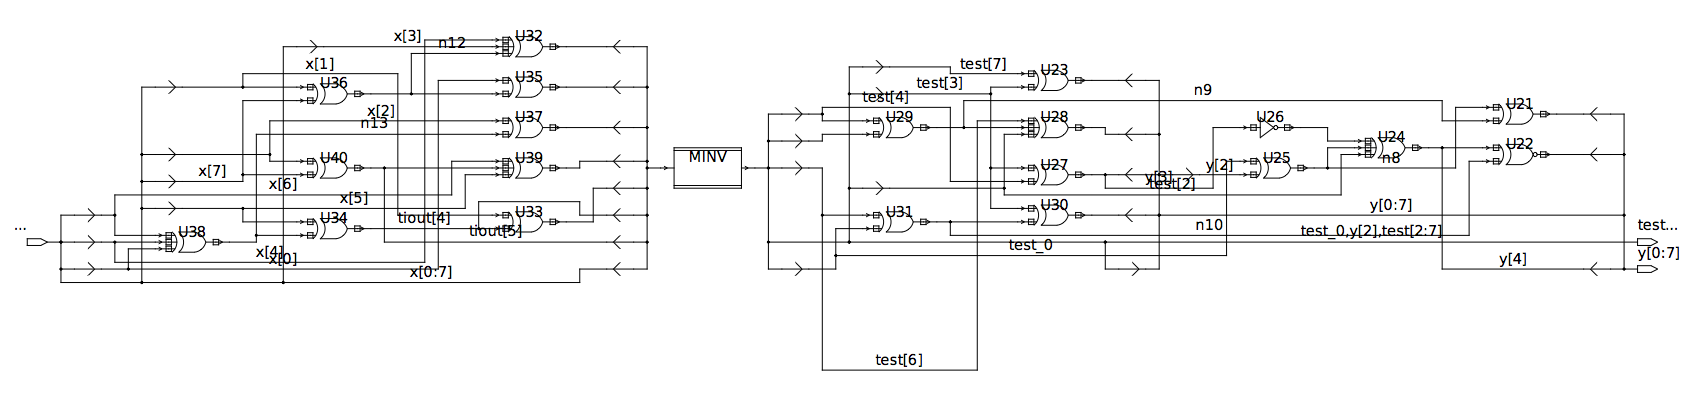
\includegraphics[scale=0.4]{./chapter_results/aes_top.png}
    % \label{fig:linearCircuita}
}
\subfigure[Top-level schematic for the inversion circuit within our overall S-box circuit.]{
    % \rule{2cm}{3cm}
    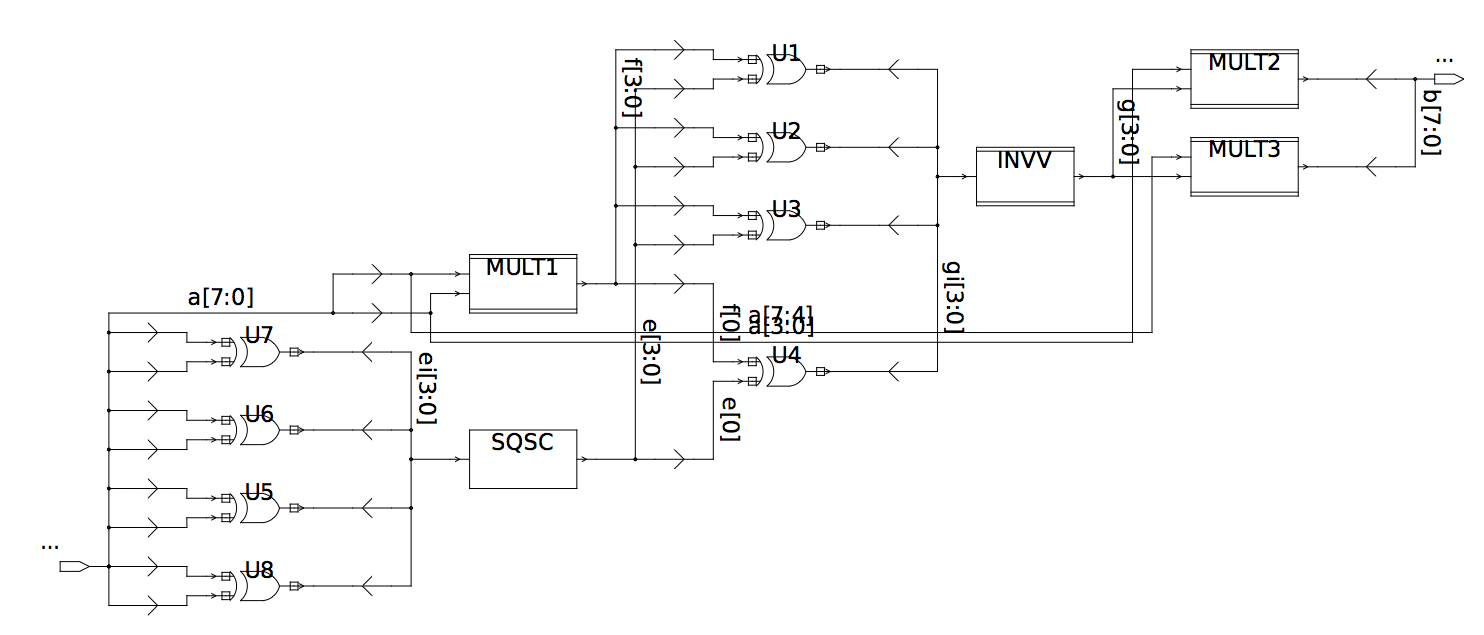
\includegraphics[scale=0.4]{./chapter_results/aes_mid.png}
    % \label{fig:linearCircuitb}
}
\caption{Schematic diagrams of the top-level schematic of the S-box and internal inversion circuit.}
\label{fig:aesAltCircuit}
\end{figure}
\end{landscape}

In addition to studying alternative irreducible polynomials that could be used to define the $GF(2^8)$ field, we also analyzed the differential uniformity and nonlinearity of all other bijective power mappings for the AES polynomial to determine if there exists suitable candidates that could be studied. These results are summarized in Table \ref{tab:gf28maps}. There are $8$ distinct power mapping exponents $d$ that yielded $\delta = 4$ and $\mathcal{N}_L = 112$. While these may be suitable candidates for the encryption step of a cryptosystem, they must be inverted in the decryption step. According to Fermat's theorem, which states that $d \times d^{-1} \equiv 1 \mod \phi(2^8)$, the inversion exponents $d^{-1}$ for each of these $8$ candidates are below:
\begin{itemize}
% \renewcommand\labelitemi{--}
 \itemsep0em
    \item $d = 127$, $d^{-1} = 253$
    \item $d = 191$, $d^{-1} = 251$
    \item $d = 223$, $d^{-1} = 247$
    \item $d = 239$, $d^{-1} = 239$
    \item $d = 247$, $d^{-1} = 223$
    \item $d = 251$, $d^{-1} = 191$
    \item $d = 253$, $d^{-1} = 127$
    \item $d = 254$, $d^{-1} = 254$
\end{itemize}

\begin{table}[ht!]
\begin{center}
\caption{Differential uniformity and nonlinearity of all bijective power mappings over $GF(2^8)$ defined by the AES irreducible polynomial $p(v) = v^8 + v^4 + v^3 + v + 1$.}
\label{tab:gf28maps}
    \begin{tabular}{|c|c|c||c|c|c||c|c|c||c|c|c|} \hline
    $d$ & $\delta$ & $\mathcal{N}_L$ & $d$ & $\delta$ & $\mathcal{N}_L$ & $d$ & $\delta$ & $\mathcal{N}_L$ & $d$ & $\delta$ & $\mathcal{N}_L$ \\ \hline
    1 & 256 & 0 & 64 & 256 & 0 & 128 & 256 & 0 & 193 & 6 & 96 \\  
    2 & 256 & 0 & 67 & 12 & 96 & 131 & 6 & 96 & 194 & 10 & 96 \\ 
    4 & 256 & 0 & 71 & 10 & 96 & 133 & 10 & 96 & 196 & 16 & 104 \\
    7 & 6 & 96 & 73 & 6 & 96 & 134 & 12 & 96 & 197 & 16 & 96 \\
    8 & 256 & 0 & 74 & 6 & 96 & 137 & 16 & 104 & 199 & 16 & 112 \\  
    11 & 10 & 96 & 76 & 16 & 104 & 139 & 16 & 96 & 202 & 30 & 80 \\ 
    13 & 12 & 96 & 77 & 16 & 96 & 142 & 10 & 96 & 203 & 16 & 104 \\  
    14 & 6 & 96 & 79 & 16 & 96 & 143 & 16 & 112 & 206 & 12 & 96 \\
    16 & 256 & 0 & 82 & 6 & 96 & 146 & 6 & 96 & 208 & 12 & 96 \\ 
    19 & 16 & 104 & 83 & 16 & 96 & 148 & 6 & 96 & 209 & 10 & 96 \\ 
    22 & 10 & 96 & 86 & 30 & 80 & 149 & 30 & 80 & 211 & 16 & 96 \\ 
    23 & 16 & 96 & 88 & 10 & 96 & 151 & 16 & 104 & 212 & 16 & 96 \\ 
    26 & 12 & 96 & 89 & 30 & 80 & 152 & 16 & 104 & 214 & 16 & 112 \\ 
    28 & 6 & 96 & 91 & 16 & 112 & 154 & 16 & 96 & 217 & 12 & 96 \\ 
    29 & 10 & 96 & 92 & 16 & 96 & 157 & 12 & 96 & 218 & 16 & 112 \\ 
    31 & 16 & 112 & 94 & 16 & 104 & 158 & 16 & 96 & {\color{red} 223} & {\color{red} 4} & {\color{red} 112} \\ 
    32 & 256 & 0 & 97 & 10 & 96 & 161 & 12 & 96 & 224 & 6 & 96 \\
    37 & 6 & 96 & 98 & 16 & 104 & 163 & 10 & 96 & 226 & 16 & 96 \\ 
    38 & 16 & 104 & 101 & 30 & 80 & 164 & 6 & 96 & 227 & 16 & 112 \\ 
    41 & 6 & 96 & 103 & 12 & 96 & 166 & 16 & 96 & 229 & 16 & 104 \\ 
    43 & 30 & 80 & 104 & 12 & 96 & 167 & 16 & 96 & 232 & 10 & 96 \\
    44 & 10 & 96 & 106 & 16 & 96 & 169 & 16 & 96 & 233 & 16 & 96 \\ 
    46 & 16 & 96 & 107 & 16 & 112 & 172 & 30 & 80 & 236 & 12 & 96 \\
    47 & 16 & 104 & 109 & 16 & 112 & 173 & 16 & 112 & {\color{red} 239} & {\color{red} 4} & {\color{red} 112} \\
    49 & 16 & 104 & 112 & 6 & 96 & 176 & 10 & 96 & 241 & 16 & 112 \\ 
    52 & 12 & 96 & 113 & 16 & 96 & 178 & 30 & 80 & 242 & 16 & 104 \\ 
    53 & 16 & 96 & 116 & 10 & 96 & 179 & 12 & 96 & 244 & 16 & 96 \\ 
    56 & 6 & 96 & 118 & 12 & 96 & 181 & 16 & 112 & {\color{red} 247} & {\color{red} 4} & {\color{red} 112} \\
    58 & 10 & 96 & 121 & 16 & 104 & 182 & 16 & 112 & 248 & 16 & 112 \\
    59 & 12 & 96 & 122 & 16 & 96 & 184 & 16 & 96 & {\color{red} 251} & {\color{red} 4} & {\color{red} 112} \\ 
    61 & 16 & 96 & 124 & 16 & 112 & 188 & 16 & 104 & {\color{red} 253} & {\color{red} 4} & {\color{red} 112} \\ 
    62 & 16 & 112 & {\color{red} 127} & {\color{red} 4} & {\color{red} 112} & {\color{red} 191} & {\color{red} 4} & {\color{red} 112} & {\color{red} 254} & {\color{red} 4} & {\color{red} 112} \\ \hline
    \end{tabular}
\end{center}
\end{table}

Therefore, both the forward and inverse exponents yield cryptographically significant power mappings. In order to determine a single candidate from these remaining exponents we analyzed their cryptographic properties using the metrics discussed in Chapter \ref{chp:motivation}. The results of this analysis are summarized in Table \ref{tab:gf28selectMapStrength}. We did not explore combinational implementations of S-boxes based on these power mappings. This is a task that may be pursued further in the future.

\begin{sidewaystable}[ht!]
\begin{center}
\caption{Differential uniformity and nonlinearity of all bijective power mappings over $GF(2^8)$ defined by the AES irreducible polynomial $p(v) = v^8 + v^4 + v^3 + v + 1$. The branch numbers are largely influenced }
\label{tab:gf28selectMapStrength}
    \begin{tabular}{|c|c|c|c|c|c|c|c|c|c|c|} \hline
    $d$ & $\mathcal{B}_n$ & $AI_c$ & $\Gamma$ (biaffine) & $\Gamma$ (quadratic) & $\Gamma'$ (biaffine) & $\Gamma'$ (quadratic) & BiAffine & Quadratic & $CI$ & Resiliency \\ \hline
    127 & 2 & 2 & 10509.45 & 7633154.49 & 86004.73 & 139884357715364.61 & 23 & 39 & 0 & 0 \\ 
    191 & 2 & 2 & 10509.45 & 7633154.49 & 86004.73 & 139884357715364.61 & 23 & 39 & 0 & 0 \\ 
    223 & 2 & 2 & 10509.45 & 7633154.49 & 86004.73 & 139884357715364.61 & 23 & 39 & 0 & 0 \\ 
    239 & 2 & 2 & 10509.45 & 7633154.49 & 86004.73 & 139884357715364.61 & 23 & 39 & 0 & 0 \\ 
    247 & 2 & 2 & 10509.45 & 7633154.49 & 86004.73 & 139884357715364.61 & 23 & 39 & 0 & 0 \\ 
    251 & 2 & 2 & 10509.45 & 7633154.49 & 86004.73 & 139884357715364.61 & 23 & 39 & 0 & 0 \\ 
    253 & 2 & 2 & 10509.45 & 7633154.49 & 86004.73 & 139884357715364.61 & 23 & 39 & 0 & 0 \\ 
    254 & 2 & 2 & 10509.45 & 7633154.49 & 86004.73 & 139884357715364.61 & 23 & 39 & 0 & 0 \\ \hline
    \end{tabular}
\end{center}
\end{sidewaystable}

\section{$16$-Bit S-Box Constructions}
Following the same methodology for finding suitable AES S-box alternatives, we considered a subset of all possible $16$-bit S-box circuits constructed using the inversion power map. Given computation both memory and computation resources for processing all mixed basis candidates, we were forced to limit our analysis. For example, it requires approximately 0.5GB of storage to hold the output from the gate counting program for a single degree $16$ irreducible polynomial over $GF(2)$. With a total of $4080$ such polynomials, this would have consumed approximately 2,040GB, or 2TB. Thus, we had to be selective in which S-boxes we examined. Also, as noted in the previous chapter, we did not consider all of the low-level algebraic optimizations of Canright because we could not programmatically check for all such optimizations. The sheer number of candidate basis selections ruled out the possibility of evaluating all cases by hand. As such, we leave such optimizations for future work, as described in Chapter \ref{chp:future}. 

For the $21$ smallest degree 16 irreducible polynomials over $GF(2)$, we identified several S-box constructions from the set of all candidates that yielded the smallest gate counts without logic optimization. Our results for each polynomial are summarized in Tables \ref{tab:rt1}, \ref{tab:rt2}, \ref{tab:rt3}, \ref{tab:rt4}, \ref{tab:rt5}, \ref{tab:rt6}, \ref{tab:rt7}, \ref{tab:rt8}, \ref{tab:rt9}, and \ref{tab:rt10} of Appendix B. Again, due to the massive number of possibilities, we did not optimize the basis change matrices shown in these tables. Here we report the best candidate for the polynomial $t(v) = v^{16} + v^5 + v^3 + v + 1$ which has a total of $1238$ XOR and $144$ AND gates. This candidate uses the basis sets $[1, V]$, $[1, W]$, $[1, X]$, $[Y^{256}, Y]$ to represent elements in $GF((((2^2)^2)^2)^2)$, where $\Sigma = v$, $\Pi = vw + v$, and $\Lambda = (vw + v)x + w$. The affine transformation and constant for this candidate shown below. Also, rather than provide a complete hardware design for this S-box, we implemented and verified it in software. The verification source code is shown in Appendix C. 

% \newpage

\begin{align*}
S(x) =  
\begin{pmatrix}
0 & 0 & 1 & 0 & 0 & 0 & 0 & 1 & 0 & 0 & 1 & 1 & 1 & 1 & 1 & 0 \\
1 & 1 & 0 & 0 & 0 & 0 & 0 & 1 & 0 & 1 & 1 & 0 & 1 & 0 & 1 & 0 \\
1 & 1 & 0 & 0 & 1 & 0 & 1 & 1 & 0 & 1 & 0 & 1 & 0 & 0 & 1 & 1 \\
1 & 1 & 1 & 0 & 0 & 0 & 1 & 0 & 0 & 1 & 1 & 0 & 0 & 0 & 0 & 0 \\
1 & 1 & 0 & 0 & 0 & 1 & 1 & 0 & 0 & 1 & 1 & 1 & 1 & 0 & 1 & 1 \\
0 & 1 & 0 & 0 & 0 & 0 & 1 & 1 & 0 & 1 & 1 & 1 & 1 & 1 & 0 & 1 \\
0 & 0 & 1 & 0 & 1 & 0 & 1 & 0 & 1 & 1 & 0 & 0 & 1 & 1 & 0 & 0 \\
1 & 0 & 1 & 1 & 1 & 0 & 1 & 1 & 0 & 0 & 0 & 1 & 0 & 1 & 1 & 1 \\
0 & 1 & 0 & 0 & 0 & 0 & 0 & 0 & 1 & 0 & 0 & 1 & 1 & 1 & 0 & 1 \\
1 & 0 & 1 & 1 & 0 & 0 & 0 & 1 & 0 & 0 & 1 & 0 & 1 & 0 & 0 & 0 \\
1 & 0 & 1 & 0 & 0 & 1 & 1 & 1 & 0 & 0 & 1 & 1 & 0 & 1 & 0 & 0 \\
1 & 0 & 1 & 1 & 1 & 0 & 1 & 1 & 1 & 1 & 0 & 1 & 1 & 0 & 0 & 1 \\
1 & 0 & 1 & 0 & 0 & 1 & 0 & 1 & 1 & 0 & 0 & 1 & 0 & 0 & 0 & 1 \\
0 & 1 & 0 & 0 & 0 & 1 & 1 & 1 & 1 & 0 & 0 & 0 & 0 & 0 & 0 & 1 \\
1 & 0 & 0 & 0 & 1 & 1 & 0 & 1 & 0 & 1 & 1 & 1 & 1 & 0 & 0 & 0 \\
1 & 1 & 0 & 1 & 0 & 1 & 1 & 0 & 1 & 0 & 0 & 1 & 1 & 0 & 0 & 0 \\
\end{pmatrix}
\begin{pmatrix}
x_{15} \\
x_{14} \\
x_{13} \\
x_{12} \\
x_{11} \\
x_{10} \\
x_{9} \\
x_{8} \\
x_{7} \\
x_{6} \\
x_{5} \\
x_{4} \\
x_{3} \\
x_{2} \\
x_{1} \\
x_{0} \\
\end{pmatrix}^{-1}
+
\begin{pmatrix}
0 \\
1 \\
0 \\
0 \\
0 \\ 
1 \\
0 \\
1 \\
1 \\
0 \\
1 \\
1 \\
0 \\ 
1 \\
1 \\
1 \\
\end{pmatrix}
% [ 0, 1, 0, 0, 0, 1, 0, 1, 1, 0, 1, 1, 0, 1, 1, 1 ]
\end{align*}
\begin{align*}
S^{-1}(x) = 
\begin{bmatrix} 
\begin{pmatrix}
0 & 1 & 0 & 1 & 0 & 1 & 1 & 1 & 0 & 0 & 1 & 0 & 0 & 0 & 0 & 1 \\
1 & 1 & 0 & 1 & 0 & 0 & 1 & 0 & 1 & 0 & 1 & 1 & 1 & 1 & 0 & 1 \\
1 & 0 & 1 & 1 & 1 & 1 & 0 & 1 & 0 & 1 & 1 & 0 & 0 & 0 & 0 & 0 \\
0 & 0 & 1 & 0 & 1 & 1 & 1 & 0 & 1 & 0 & 1 & 1 & 1 & 0 & 1 & 0 \\
1 & 1 & 1 & 1 & 1 & 0 & 0 & 0 & 1 & 0 & 0 & 0 & 0 & 1 & 0 & 0 \\
0 & 0 & 0 & 1 & 0 & 1 & 0 & 0 & 0 & 0 & 1 & 1 & 1 & 1 & 1 & 1 \\
1 & 0 & 1 & 0 & 0 & 0 & 0 & 0 & 0 & 1 & 1 & 0 & 1 & 0 & 1 & 1 \\
0 & 0 & 1 & 0 & 1 & 1 & 1 & 0 & 0 & 1 & 0 & 1 & 1 & 1 & 1 & 0 \\
0 & 0 & 0 & 0 & 0 & 0 & 1 & 0 & 0 & 0 & 1 & 0 & 0 & 0 & 1 & 0 \\
1 & 1 & 1 & 0 & 0 & 1 & 1 & 1 & 1 & 0 & 1 & 1 & 1 & 0 & 0 & 0 \\
0 & 1 & 1 & 0 & 1 & 1 & 1 & 1 & 0 & 0 & 1 & 0 & 1 & 1 & 1 & 1 \\
1 & 0 & 0 & 1 & 1 & 0 & 0 & 0 & 1 & 0 & 0 & 1 & 1 & 0 & 1 & 1 \\
1 & 0 & 0 & 0 & 0 & 1 & 0 & 1 & 1 & 1 & 0 & 0 & 1 & 0 & 1 & 0 \\
1 & 0 & 0 & 0 & 0 & 1 & 1 & 1 & 1 & 1 & 0 & 1 & 1 & 1 & 1 & 1 \\
1 & 1 & 1 & 0 & 0 & 1 & 1 & 0 & 1 & 0 & 0 & 1 & 1 & 1 & 1 & 1 \\
0 & 1 & 0 & 0 & 1 & 0 & 1 & 0 & 1 & 0 & 0 & 1 & 0 & 0 & 0 & 1 \\
\end{pmatrix}
\begin{pmatrix}
x_{15} \\
x_{14} + 1 \\
x_{13} \\
x_{12} \\
x_{11} \\
x_{10} + 1 \\
x_{9} \\
x_{8} + 1 \\
x_{7} + 1 \\
x_{6} \\
x_{5} + 1 \\
x_{4} + 1 \\
x_{3} \\
x_{2} + 1 \\
x_{1} + 1 \\
x_{0} + 1 \\
\end{pmatrix}
\end{bmatrix}^{-1}
\end{align*}

\newpage 

The basis change matrices used in this S-box candidate are shown below. 

\begin{align*}
\mathbf{T} = 
\begin{pmatrix}
0 &1 &0 &1 &0 &0 &0 &0 &1 &0 &0 &0 &0 &1 &0 &0\\
0 &1 &1 &0 &0 &1 &1 &1 &0 &0 &1 &0 &0 &1 &1 &1\\
0 &0 &0 &1 &1 &0 &0 &1 &0 &0 &0 &1 &0 &0 &0 &1\\
1 &1 &0 &0 &0 &0 &1 &1 &0 &1 &0 &1 &0 &0 &1 &1\\
1 &1 &0 &0 &1 &0 &0 &1 &0 &0 &0 &1 &0 &1 &0 &1\\
0 &0 &1 &1 &0 &1 &1 &1 &1 &0 &0 &0 &1 &0 &0 &1\\
0 &0 &0 &1 &1 &0 &1 &0 &1 &0 &1 &0 &0 &1 &0 &0\\
0 &0 &1 &0 &1 &0 &1 &0 &0 &1 &1 &1 &0 &1 &0 &0\\ 
1 &0 &1 &0 &0 &1 &1 &1 &1 &0 &1 &1 &0 &0 &1 &1\\
0 &0 &0 &1 &0 &1 &0 &1 &0 &1 &1 &0 &0 &1 &0 &1\\
1 &1 &0 &1 &1 &0 &1 &1 &0 &0 &1 &0 &0 &0 &0 &1\\
0 &1 &1 &1 &0 &1 &0 &0 &1 &1 &1 &0 &0 &0 &1 &0\\
0 &1 &0 &1 &1 &1 &0 &0 &1 &1 &0 &1 &0 &0 &0 &0\\
1 &0 &0 &1 &0 &0 &0 &0 &0 &0 &1 &0 &0 &1 &0 &0\\
0 &1 &0 &0 &0 &1 &0 &0 &0 &1 &0 &1 &0 &0 &1 &0\\
0 &1 &0 &0 &0 &0 &1 &1 &1 &0 &1 &1 &0 &0 &0 &0\\
\end{pmatrix}
\end{align*}
\begin{align*}
\mathbf{T}^{-1} = 
\begin{pmatrix}
1 &0 &1 &0 &0 &0 &0 &1 &1 &0 &0 &0 &0 &0 &1 &0\\
1 &0 &0 &0 &1 &0 &0 &0 &0 &1 &0 &0 &1 &1 &0 &0\\
1 &1 &0 &0 &1 &0 &0 &0 &1 &1 &0 &1 &1 &0 &1 &0\\
0 &1 &1 &1 &1 &0 &1 &1 &1 &0 &1 &1 &1 &0 &0 &0\\
0 &0 &0 &1 &1 &0 &0 &1 &0 &0 &0 &1 &1 &0 &0 &0\\
0 &1 &0 &1 &1 &0 &1 &0 &1 &0 &0 &0 &0 &1 &1 &0\\
1 &0 &1 &1 &0 &0 &1 &1 &0 &0 &0 &1 &1 &1 &0 &0\\
1 &0 &0 &0 &1 &0 &0 &0 &0 &0 &1 &0 &0 &0 &0 &1\\
0 &0 &0 &0 &1 &0 &0 &1 &1 &0 &0 &0 &0 &0 &1 &0\\
1 &0 &1 &0 &0 &0 &1 &1 &0 &1 &0 &1 &1 &0 &1 &0\\
1 &0 &1 &0 &0 &0 &0 &0 &0 &1 &0 &0 &1 &0 &0 &0\\
0 &0 &0 &1 &1 &0 &1 &0 &1 &0 &1 &1 &1 &0 &1 &0\\
0 &0 &0 &0 &1 &1 &1 &1 &0 &1 &1 &0 &0 &0 &0 &0\\
0 &1 &1 &1 &1 &0 &1 &0 &0 &1 &1 &1 &0 &1 &1 &0\\
0 &1 &1 &0 &1 &0 &1 &1 &0 &0 &1 &0 &1 &0 &0 &0\\
1 &1 &0 &1 &0 &0 &0 &0 &0 &0 &1 &1 &1 &0 &1 &1\\
\end{pmatrix}
\end{align*}

In the current state of this work, we are optimizing all 165,888 basis combinations on the Open Science Grid \cite{Sfiligoi09-1} \cite{Pordes2008}. Future work will consist of using these results to present an S-box candidate with an even smaller gate count.
